\begin{exercises} 

\item \label{Ez:10.3.0}   Shown in Figure \ref{F:10.3.activity.contour} is a contour
  plot of a function $f$ with the values of $f$ labeled on the
  contours.  The point $(2,1)$ is highlighted in red. 

\begin{figure}[ht]
  \begin{center}
    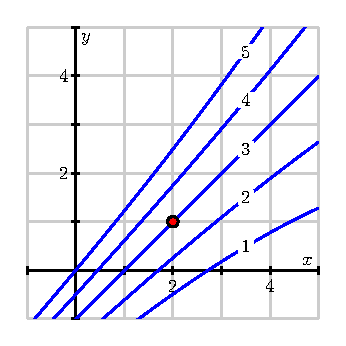
\includegraphics{figures/fig_10_3_activity_contour.eps}
    \caption{A contour plot of $f(x,y)$.}
    \label{F:10.3.activity.contour}
  \end{center}
\end{figure}

\ba
\item Estimate the partial derivatives $f_x(2,1)$ and $f_y(2,1)$.
\item Determine whether the second-order partial derivative
  $f_{xx}(2,1)$ is positive or negative, and explain your thinking. 
\item Determine whether the second-order partial derivative
  $f_{yy}(2,1)$ is positive or negative, and explain your thinking.
\item Determine whether the second-order partial derivative
  $f_{xy}(2,1)$ is positive or negative, and explain your thinking.
\item Determine whether the second-order partial derivative
  $f_{yx}(2,1)$ is positive or negative, and explain your thinking.
\item Consider a function $g$ of the variables $x$ and $y$ for which $g_x(2,2) > 0$ and
  $g_{xx}(2,2) < 0$.  Sketch possible behavior of some contours around $(2,2)$ on the left axes in Figure \ref{F:10.3.activity.grad}.
  \begin{figure}[ht]
    \begin{center}
      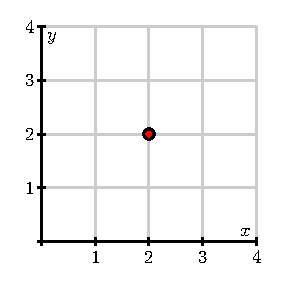
\includegraphics{figures/fig_10_2_activity_grad.eps}
      \hspace*{1in}
      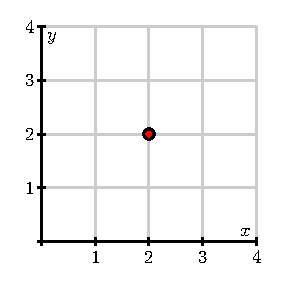
\includegraphics{figures/fig_10_2_activity_grad.eps}
    \end{center}
    \caption{Plots for contours of $g$ and $h$.}
    \label{F:10.3.activity.grad}
  \end{figure}
\item Consider a function $h$ of the variables $x$ and $y$ for which $h_x(2,2) > 0$ and
  $h_{xy}(2,2) < 0$.  Sketch possible behavior of some contour
  lines around $(2,2)$ on the right axes in Figure \ref{F:10.3.activity.grad}.

\ea

\begin{exerciseSolution}
\ba
\item Approximating the partial derivatives with difference quotients gives us
\[f_x(2,1) \approx \frac{f(3,1)-f(1,1)}{2} \approx \frac{2-4.8}{2} = -1.4\]
and
\[f_y(2,1) \approx \frac{f(2,2)-f(2,0)}{2} \approx \frac{4.3-1.8}{2} = 1.25.\] 
\item The contours appear to be more spread out as $x$ increases from the point $(2,1)$, indicating a more level surface. Since $f_x(2,1) < 0$ and the slopes in the $x$-direction are getting closer to 0, it must be that $f_{x}$ is increasing. So $f_{xx}(2,1)$ should be positive. This is reinforced by the approximation 
\[f_x(3,1) \approx \frac{f(4,1)-f(2,1)}{2} \approx \frac{1.2-3}{2} = -0.9 > f_x(2,1).\]
\item The contours appear to be closer together as $y$ increases from the point $(2,1)$, indicating a steeper surface. Since $f_y(2,1) > 0$ and the slopes in the $y$-direction are getting larger, it must be that $f_{y}$ is increasing. So $f_{yy}(2,1)$ should be positive. This is reinforced by the approximation
\[f_2(2,2) \approx \frac{f(2,2.5)-f(2,1.5)}{1} \approx 5-3.7 = 1.3 > f_y(2,1).\]
\item Recall that $f_{xy} = (f_x)_y$ tells us how the slopes of tangent lines to the surface in the $x$ direction change as $y$ increases. It appears that as we increase $y$ from $(1,2)$ the contours are more closely spaced, indicating a greater magnitude change in $z$ for a given change in $x$. But since $f_x(2,1) < 0$, we should expect that $f_{x}$ is getting more negative as $y$ increases and that $f_{xy}$ is negative. This is reinforced by the fact that 
\[f_x(2,2) \approx \frac{f(2.5,2)-f(1.5,2)}{1} \approx  = 3.5-5 = -1.5 < f_x(2,1).\]

\item Recall that $f_{yy} = (f_y)_x$ tells us how the slopes of tangent lines to the surface in the $y$ direction change as $x$ increases. It appears that as we increase $x$ from $(1,2)$ the contours are spaced farther apart, indicating a decrease in magnitude change in $z$ for a given change in $y$. The fact that $f_y(2,1) > 0$ tells us that we should expect $f_{y}$ to be getting smaller as $x$ increases and that $f_{yx}$ is negative. This is reinforced by the fact that 
\[f_y(3,1) \approx \frac{f(3,2)-f(3,0)}{2} \approx \frac{3-1.2}{2} = 0.9 < f_y(2,1).\] 
\item If $g_x(2,2)> 0$ and $g_{xx}(2,2) < 0$, the slopes of the tangent lines in the $x$ direction will be getting smaller as $x$ increases from the point $(2,2)$.  This implies that the surface will be leveling out in the $x$ direction from this point and so the contours will be spaced farther apart in the $x$ direction. An example would be $g(x,y) = -\frac{1}{2^x}$. 
\item If $h_x(2,2)> 0$ and $h_{xy}(2,2) = (h_x)_y(2,2) < 0$, the slopes of the tangent lines in the $x$ direction will be getting smaller as $y$ increases from the point $(2,2)$. This implies that the surface will be leveling out in the $y$ direction from this point and so the contours will be spaced farther apart in the $x$ direction as $y$ increases. An example would be $h(x,y) = 2x^2-2xy$.  

\ea
\end{exerciseSolution}



\item \label{Ez:10.3.1}   The Heat Index, $I$, (measured in \emph{apparent degrees F}) is a function of the actual temperature $T$ outside (in degrees F) and the relative humidity $H$ (measured as a percentage).  A portion of the table which gives values for this function, $I(T,H)$, is reproduced below:
\begin{center}
\begin{tabular}{|l||r|r|r|r|} \hline
\emph{T} $\downarrow \backslash$ \emph{H} $\rightarrow$ & 70 &	75 & 80 &	85  \\ \hhline{|=|=|=|=|=|}
90 & 106 & 109 & 112 & 115  \\ \hline
92 & 112 & 115 & 119 & 123  \\ \hline
94 & 118 & 122 & 127 & 132  \\ \hline
96 & 125 & 130 & 135 & 141  \\ \hline
\end{tabular}
\end{center}

				
    \ba
   	\item State the limit definition of the value $I_{TT}(94,75)$.  Then, estimate $I_{TT}(94,75)$, and write one complete sentence that carefully explains the meaning of this value, including units.	
	

	\item State the limit definition of the value $I_{HH}(94,75)$.  Then, estimate $I_{HH}(94,75)$, and write one complete sentence that carefully explains the meaning of this value, including units.
	
	\item Finally, do likewise to estimate $I_{HT}(94,75)$, and write a sentence to explain the meaning of the value you found.
	
   \ea
   

\begin{exerciseSolution}
    \ba
   	\item The limit definition of $I_{TT}(94,75)$ is
\[I_{TT}(94,75) = \lim_{h \to 0} \frac{I_T(94+h,75)-I_T(94,75)}{h}.\]
To estimate  $I_{TT}(94,75)$ we will use the symmetric difference quotient 
\[I_{TT}(94,75) \approx \frac{I_T(96,75) - I_T(92,75)}{4}.\]
To do this we need to approximate $I_T(96,75)$ and $I_T(92,75)$. For $I_T(96,75)$ we can only use a backwards difference quotient, but for $I_T(92,75)$ we can use asymmetric difference quotient:
\[I_T(96,75) \approx \frac{I(96,75)-I(94,75)}{2} = 3.5 \ \text{ and } \ I_T(92,75) \approx \frac{I(94,75)-I(90,75)}{4} = 3.\]
Thus,
\[I_{TT}(94,75) \approx \frac{3.5 - 3}{4} = 0.125 \ \frac{\frac{\text{apparant }^{\circ}\text{F}}{^{\circ}\text{F}}}{^{\circ}\text{F}}.\]
The fact that $I_{TT}(94,75) \approx 0.125$ means that for every one $^{\circ}F$ increase in temperature from $94^{\circ}$F, the rate at which the heat index changes as the temperature increases grows by approximately 0.125 $\frac{\text{apparant }^{\circ}F}{^{\circ}F}$ if the relative humidity is held at 75\%. In other words, $I_{T}(95,75)$ is approximately 0.125 greater than $I_{T}(94,75)$. 


	\item The limit definition of $I_{HH}(94,75)$ is
\[I_{HH}(94,75) = \lim_{h \to 0} \frac{I_H(94,75+h)-I_H(94,75)}{h}.\]
To estimate  $I_{HH}(94,75)$ we will use the symmetric difference quotient 
\[I_{HH}(94,75) \approx \frac{I_H(94,80) - I_T(94,70)}{10}.\]
To do this we need to approximate $I_H(94,80)$ and $I_H(94,70)$. For $I_H(94,70)$ we can only use a forward difference quotient, but for $I_H(94,80)$ we can use asymmetric difference quotient:
\[I_H(94,70) \approx \frac{I(94,75)-I(94,70)}{5} = 0.8 \ \text{ and } \ I(94,80) \approx \frac{I(94,85)-I(90,75)}{10} = 1.\]
Thus,
\[I_{HH}(94,75) \approx \frac{1 - 0.8}{10} = 0.02 \ \frac{ \frac{\text{apparant }^{\circ}\text{F}}{\% \text{ Humidity}} }{\% \text{ Humidity}}.\]
The fact that $I_{HH}(94,75) \approx 0.02$ means that for every one \% increase in the relative humidity from 75\%, the rate at which the heat index changes as the relative humidity increases grows by approximately 0.02 $\frac{\text{apparant }^{\circ}F}{\% \text{ Humidity}}$ if the temperature is held constant at $94^{\circ}$F. In other words, $I_{H}(94,76)$ is approximately 0.02 greater than $I_{H}(94,75)$. 
	
	\item The limit definition of $I_{HT}(94,75)$ is
\[I_{HT}(94,75) = \lim_{h \to 0} \frac{I_H(94+h,75)-I_H(94,75)}{h}.\]
To estimate  $I_{HT}(94,75)$ we will use the symmetric difference quotient 
\[I_{HT}(94,75) \approx \frac{I_H(96,75) - I_H(92,75)}{4}.\]
To do this we need to approximate $I_H(96,75)$ and $I_H(92,75)$. For both we use a symmetric difference quotient:
\[I_H(96,75) \approx \frac{I(96,80)-I(96,70)}{10} = 0.9 \ \text{ and } \ I_H(92,75) \approx \frac{I(92,80)-I(92,70)}{10} = 0.7.\]
Thus,
\[I_{HT}(94,75) \approx \frac{0.9 - 0.7}{4} = 0.05 \ \frac{\frac{\text{apparant }^{\circ}\text{F}}{\% \text{ Humidity}} }{^{\circ}\text{F}}.\]
The fact that $I_{HT}(94,75) \approx 0.05$ means that for every one degree increase in temperature from $94^{\circ}$F, the rate at which the heat index changes as the relative humidity increases grows by approximately 0.05 $\frac{\text{apparant }^{\circ}F}{\% \text{ Humidity}}$.   In other words, $I_{H}(95,75)$ is approximately 0.05 greater than $I_{H}(94,75)$. 
	
   \ea
\end{exerciseSolution}


\item \label{Ez:10.3.2}   The temperature on a heated metal plate positioned in the first quadrant of the $x$-$y$ plane is given by 
$$C(x,y) = 25e^{-(x-1)^2 - (y-1)^3}.$$
Assume that temperature is measured in degrees Celsius and that $x$ and $y$ are each measured in inches. 
\ba

	\item Determine $C_{xx}(x,y)$ and $C_{yy}(x,y)$.  Do not do any additional work to algebraically simplify your results.

	\item Calculate $C_{xx}(1.1, 1.2)$.  Suppose that an ant is walking past the point $(1.1, 1.2)$ along the line $y = 1.2$.  Write a sentence to explain the meaning of the value of $C_{xx}(1.1, 1.2)$, including units.  

	\item Calculate $C_{yy}(1.1, 1.2)$.  Suppose instead that an ant is walking past the point $(1.1, 1.2)$ along the line $x = 1.1$.  Write a sentence to explain the meaning of the value of $C_{yy}(1.1, 1.2)$, including units.
	
	\item Determine $C_{xy}(x,y)$ and hence compute $C_{xy}(1.1, 1.2)$.  What is the meaning of this value?  Explain, in terms of an ant walking on the heated metal plate.

\ea


\begin{exerciseSolution}
\ba

	\item First we find $C_x$ and $C_y$:
\[C_x(x,y) = 25e^{-(x-1)^2 - (y-1)^3}\left(-2(x-1)\right) \ \text{ and } \ C_y(x,y) = 25e^{-(x-1)^2 - (y-1)^3}\left(-3(y-1)^2\right).\]
Then
\begin{align*}
C_{xx}(x,y) &= -50e^{-(x-1)^2 - (y-1)^3} + \left(-2(x-1)\right)\left(25e^{-(x-1)^2 - (y-1)^3}\left(-2(x-1)\right)\right) \\
C_{yy}(x,y) &= -150(y-1)e^{-(x-1)^2 - (y-1)^3} + \left(-3(y-1)^2\right)\left(25e^{-(x-1)^2 - (y-1)^3}\left(-3(y-1)\right)\right).
\end{align*}


	\item Using the result of part (a) we have 
\[C_{xx}(1.1, 1.2) \approx -48.13 \ \frac{\frac{^{\circ}\text{C}}{\text{in}}}{\text{in}}.\]
When the ant is walking along the line $y=1.2$, for every inch the ant moves from $x=1.1$ in the positive direction, the rate at which the temperature is changing for each inch traveled in the positive $x$ direction is decreasing by approximately 48.13 $\frac{^{\circ}C}{\textbf{in}}$. 

	\item Using the result of part (a) we have 
\[C_{yy}(1.1, 1.2) \approx -29.11 \ \frac{\frac{^{\circ}\text{C}}{\text{in}}}{\text{in}}.\]
When the ant is walking along the line $x=1.1$, for every inch the ant moves from $y=1.2$ in the positive direction, the rate at which the temperature is changing for each inch traveled in the positive $y$ direction is decreasing by approximately 29.11 $\frac{^{\circ}C}{\textbf{in}}$. 
	
	\item Differentiating $C_x(x,y)$ with respect to $y$ yields
\[C_{xy}(x,y) = -50(x-1)e^{-(x-1)^2 - (y-1)^3}\left(-3(y-1)^2\right).\]
So
\[C_{xy}(1.1, 1.2) \approx 0.59 \ \frac{\frac{^{\circ}\text{C}}{\text{in}}}{\text{in}}.\]
For every inch the ant moves from $(1.1,1.2)$ in the positive $y$ direction, the rate at which the temperature is changing for each inch traveled in the positive $x$ direction is increasing by approximately 0.59 $\frac{^{\circ}C}{\textbf{in}}$. 


\ea


\end{exerciseSolution}



\item \label{Ez:10.3.3}  Let $f(x,y) = 8 - x^2 - y^2$ and $g(x,y) = 8 - x^2 + 4xy - y^2$.
				
    \ba
   	\item Determine $f_x$, $f_y$, $f_{xx}$, $f_{yy}$, $f_{xy}$, and $f_{yx}$.
	\item Evaluate each of the partial derivatives in (a) at the point $(0,0)$.
	\item What do the values in (b) suggest about the behavior of $f$ near $(0,0)$?  Plot a graph of $f$ and compare what you see visually to what the values suggest.
	\item Determine $g_x$, $g_y$, $g_{xx}$, $g_{yy}$, $g_{xy}$, and $g_{yx}$.
	\item Evaluate each of the partial derivatives in (d) at the point $(0,0)$.
	\item What do the values in (e) suggest about the behavior of $g$ near $(0,0)$?  Plot a graph of $g$ and compare what you see visually to what the values suggest.
	\item What do the functions $f$ and $g$ have in common at $(0,0)$?  What is different?  What do your observations tell you regarding the importance of a certain second-order partial derivative?
	 
    \ea


\begin{exerciseSolution}
    \ba
   	\item Using the standard differentiation rules gives us
\begin{align*}
f_x(x,y) &= -2x \\
f_y(x,y) &= -2y \\
f_{xx}(x,y) &= -2 \\
f_{yy}(x,y) &= -2 \\
f_{xy}(x,y) &= 0 \\
f_{yx}(x,y) &= 0.
\end{align*}

	\item Evaluating at $(0,0)$ we find that
\begin{align*}
f_x(0,0) &= 0 \\
f_y(0,0) &= 0 \\
f_{xx}(0,0) &= -2 \\
f_{yy}(0,0) &= -2 \\
f_{xy}(0,0) &= 0 \\
f_{yx}(0,0) &= 0.
\end{align*}.
	\item The fact that the first order partial derivatives are 0 at $(0,0)$ indicates that the surface is flat in the $x$ and $y$ directions around $(0,0)$, while the unmixed partials indicate that the surface is concave down in the $x$ and $y$ directions. The mixed partials suggest that the is no twist to the surface in either the $x$ or $y$ direction at $(0,0)$. All of this information implies that the surface looks bowl-shaped at $(0,0)$.  
	\item Using the standard differentiation rules gives us
\begin{align*}
g_x(x,y) &= -2x+4y \\
g_y(x,y) &= 4x-2y \\
g_{xx}(x,y) &= -2 \\
g_{yy}(x,y) &= -2 \\
g_{xy}(x,y) &= 4 \\
g_{yx}(x,y) &= 4.
\end{align*}

	\item Evaluating at $(0,0)$ we find that
\begin{align*}
g_x(0,0) &= 0 \\
g_y(0,0) &= 0 \\
g_{xx}(0,0) &= -2 \\
g_{yy}(0,0) &= -2 \\
g_{xy}(0,0) &= 4 \\
g_{yx}(0,0) &= 4.
\end{align*}.
	\item The fact that the first order partial derivatives are 0 at $(0,0)$ indicates that the surface is flat in the $x$ and $y$ directions around $(0,0)$, while the unmixed partials indicate that the surface is concave down in the $x$ and $y$ directions. The mixed partials suggest that the is a positive  twist to the surface in both the $x$ and $y$ directions at $(0,0)$. All of this information implies that the surface looks like a saddle at $(0,0)$.  
	\item The two surfaces are alike in that they are both flat in the $x$ and $y$ directions around $(0,0)$, while the unmixed partials indicate that the surfaces are concave down in the $x$ and $y$ directions. The difference is in the second order mixed partials that produce a twist in $g$ but no twist in $f$ at $(0,0)$. This accounts for the different shapes of the surfaces. 
    \ea
\end{exerciseSolution}


\item Let $f(x,y) = \frac{1}{2}xy^2$ represent the kinetic energy in Joules of an object of mass $x$ in
kilograms with velocity $y$ in meters per second. Let $(a,b)$ be the point $(4,5)$ in the domain of $f$.
	\ba
	\item Calculate $\ds \frac{ \partial^2 f}{\partial x^2}$ at the point $(a,b)$. Then explain as best you can what this second order partial
derivative tells us about kinetic energy. %(Hint: Recall that $\ds \frac{ \partial^2 f}{\partial x^2}$ is the second order unmixed partial derivative of
%$f_x$ with respect to $x$ as discussed in Activity \ref{act:10.2.5}.)

	\item Calculate $\ds \frac{ \partial^2 f}{\partial y^2}$ at the point $(a,b)$. Then explain as best you can what this second order partial
derivative tells us about kinetic energy.

	\item Calculate $\ds \frac{ \partial^2 f}{\partial y \partial x}$ at the point $(a,b)$. Then explain as best you can what this second order
partial derivative tells us about kinetic energy.

	\item Calculate $\ds \frac{ \partial^2 f}{\partial x \partial y}$ at the point $(a,b)$. Then explain as best you can what this second order
partial derivative tells us about kinetic energy.

	\ea

\begin{exerciseSolution}
\ba
\item Since $f_x(x,y) = \frac{1}{2}y^2$, we have 
\[\frac{ \partial^2 f}{\partial x^2}  = 0.\]
So $f_{xx}(a,b) = 0$.  This calculation tells us that a small increase in the mass of an object from 4 kg does not affect the rate at which the kinetic energy changes as we increase the mass. In other words, $\frac{\partial f}{\partial x}(4.1,5)$ should be approximately the same as $\frac{\partial f}{\partial x}(4,5)$ 

\item Since $f_y(x,y) = xy$, we have 
\[\frac{ \partial^2 f}{\partial y^2}  = x.\]
So $f_{yy}(a,b) = 4$.  This calculation tells us that increasing the velocity of an object by one meter per second from 5 meters per second while keeping the mass constant at 4 kg causes an approximate 4 unit (in Joules per meter per second) increase in the rate at which the kinetic energy changes as we increase the velocity. In other words, $\frac{\partial f}{\partial y}(4,6)$ should be approximately $4$ Joules per meters per second larger than $\frac{\partial f}{\partial y}(4,5)$.  

\item Since  
\[\frac{ \partial^2 f}{\partial y \partial x}  = y,\]
we have $f_{xy}(a,b) = 5$.  This calculation tells us that increasing the mass of an object by one kg from 4 kg while keeping the velocity constant at 5 meters per second causes an approximate 5 unit (in Joules per kilogram) increase in the rate at which the kinetic energy changes as we increase the mass. In other words, $\frac{\partial f}{\partial x}(4,6)$ should be approximately $5$ Jules per kilogram larger than $\frac{\partial f}{\partial x}(4,5)$.  

\item Since  
\[\frac{ \partial^2 f}{\partial x \partial y}  = y,\]
we have $f_{yx}(a,b) = 5$.  This calculation tells us that increasing the velocity of an object by one meter per second from 5 meters per second while keeping the mass constant at 4 kg causes an approximate 5 unit (in Joules per meter per second) increase in the rate at which the kinetic energy changes as we increase the velocity. In other words, $\frac{\partial f}{\partial y}(5,5)$ should be approximately $5$ Jules per meter per second larger than $\frac{\partial f}{\partial y}(4,5)$.  
\ea
\end{exerciseSolution}

\end{exercises}
\afterexercises
